\chapter{Background}
This chapter describes relevant technical background and relevant work. We will first define the field of machine learning, and then describe the methods that have been used in this thesis. We will explain feature extraction for audio signals using spectrograms. We will also describe recent relevant work that uses the same machine learning methods and feature extractions methods as in this thesis.
\section{Machine learning}
%http://publications.idiap.ch/downloads/papers/2015/Revaz_THESIS_2015.pdf
%hva er det (for dummies)%
Donec id massa ac leo consequat euismod et a sem. Pellentesque sem justo, vulputate vel neque a, ultrices dapibus ipsum. Vestibulum orci orci, semper ut odio et, luctus condimentum nunc.
\cite{Esteva2017}.Mauris vel interdum nunc. Curabitur mi lectus, rhoncus venenatis ullamcorper quis, mattis volutpat dui. Proin at lectus ac metus ornare lacinia et pretium risus \cite{Homesite2017}.
%Some of the most
\subsubsection{Accuracy}

$$ \text{Accuracy} = \frac{TP + TN}{P+N}$$
Aenean rhoncus, nisi in suscipit aliquet, eros diam tempus nunc, non luctus turpis mauris ut lorem. Nulla sed scelerisque mauris.
\subsubsection{Recall}
Aenean rhoncus, nisi in suscipit aliquet, eros diam tempus nunc, non luctus turpis mauris ut lorem. Nulla sed scelerisque mauris.
$$ \text{Recall}= \frac{TP}{TP + FN}$$
Aenean rhoncus, nisi in suscipit aliquet, eros diam tempus nunc, non luctus turpis mauris ut lorem. Nulla sed scelerisque mauris.
\subsubsection{Precision}

\section{Deep learning}
\subsection{Convolutional neural network}
Aenean rhoncus, nisi in suscipit aliquet, eros diam tempus nunc, non luctus turpis mauris ut lorem. Nulla sed scelerisque mauris. Figure \ref{fig:cnn_layer} shows an illustration of the convolutional layer.

\begin{figure}[h]
\begin{center}
  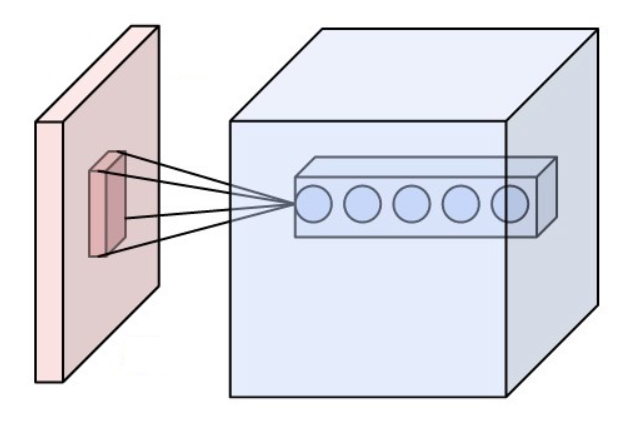
\includegraphics[width=3in]{../fig/cnn_conv.png}
  \caption{Illustration of the convolutional layer . The red box is the input, and blue box is the result. The width and height of the input is preserved, but since the convolutional filter has 32 filters, the depth of the output volume is 32 pixels.}
  \label{fig:cnn_layer}
\end{center}
\end{figure}

\section{Classification vs. detection}
\label{sec:object_detection}


\begin{figure}[h]
  \begin{subfigure}[b]{0.245\textwidth}
    \centering
    \textbf{Classification}\par\medskip
    \includegraphics[width=\textwidth]{../fig/cat.jpg}
    \caption{Cat}
    \label{fig:CatOne}
  \end{subfigure}
  %\quad
  \begin{subfigure}[b]{0.245\textwidth}
    \centering
    \textbf{Localization}\par\medskip
    \includegraphics[width=\textwidth]{../fig/cat_localization.jpg}
    \caption{Cat}
    \label{fig:CatTwo}
  \end{subfigure}
  %\quad
 \begin{subfigure}[b]{0.245\textwidth}
   \centering
   \textbf{Detection}\par\medskip
    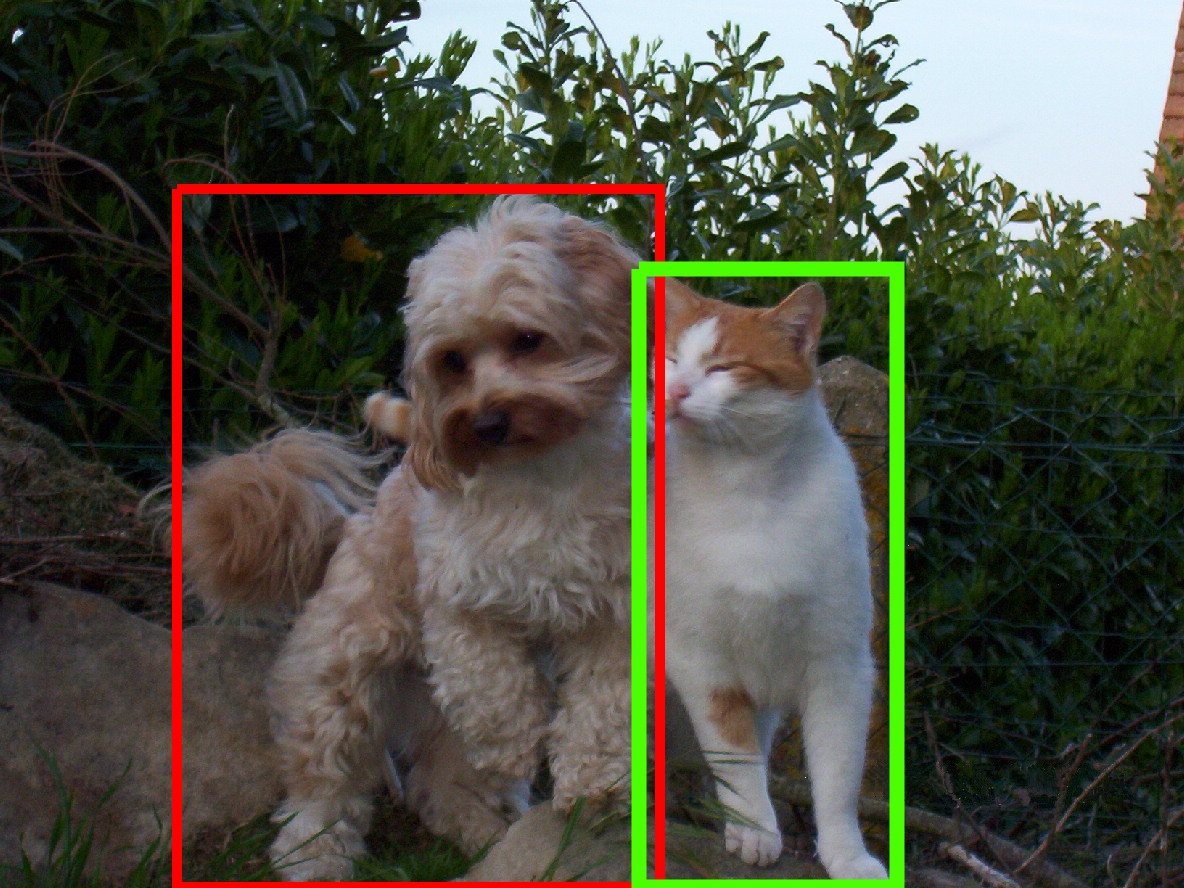
\includegraphics[width=\textwidth]{../fig/cat_dog_detection.jpg}
    \caption{Cat, Dog}
    \label{fig:CatDogOne}
  \end{subfigure}
  %\quad
  \begin{subfigure}[b]{0.245\textwidth}
    \centering
    \textbf{Segmentation}\par\medskip
     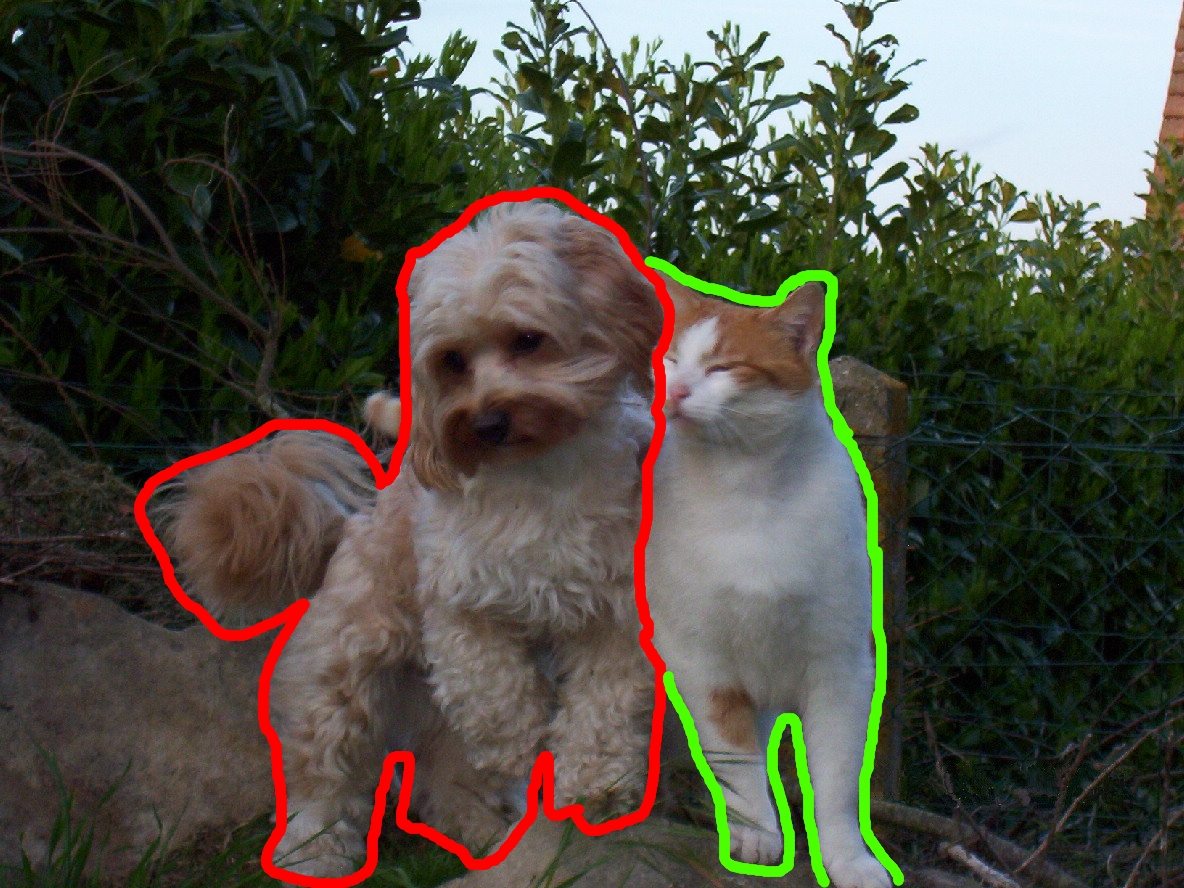
\includegraphics[width=\textwidth]{../fig/cat_dog_segmentation.jpg}
     \caption{Cat, Dog}
     \label{fig:CatDogTwo}
   \end{subfigure}
  \caption{Vizualisation of four different image recognition tasks }
  \label{fig:class_det}
\end{figure}

\begin{itemize}
\item \textbf{Classification:} Donec id massa ac leo consequat euismod et a sem. Pellentesque sem justo, vulputate vel neque a, ultrices dapibus ipsum. Vestibulum orci orci, semper ut odio et, luctus condimentum nunc.
\item \textbf{Object localization:} Donec id massa ac leo consequat euismod et a sem. Pellentesque sem justo, vulputate vel neque a, ultrices dapibus ipsum. Vestibulum orci orci, semper ut odio et, luctus condimentum nunc.  the size of the bounding box.
\item \textbf{Object detection:}Donec id massa ac leo consequat euismod et a sem. Pellentesque sem justo, vulputate vel neque a, ultrices dapibus ipsum. Vestibulum orci orci, semper ut odio et, luctus condimentum nunc.

\end{itemize}
